\subsection{Experiment}
\subsubsection{Site and Borehole Heat Exchanger}
	%District system, estimated total demand to be satisified.
	Need for geothermal district heating/cooling demand for potentially the entire campus. It is crucial to assess the possibilities of using deeper geothermal heat exchangers.

	%Drilling
	The drilling of the well took place beginning August 8th, 2019. To characterize the formation layering at the drill site, a geological survey was performed immediately after the drilling. On top of
	The drilling of the site identified began on August 12th, 2019, and encountered significant amount of underground water upon reaching approximately 150 feet (45.7 meters) depth. The composition of the ground was primarily sand stone and mudstone until hitting gravel at approximately 1000 feet (300 meters) depth. The remainder of the drilling to approximately 1400 feet (430 meters) took significantly longer, and appeared to have hit quartz and hence halted the drilling of the test bore at 1440 feet the subsequent day. USGS (United States Geological Survey) performed a geophysics survey on the test bore immediately after the drillers pulled out, and determined similar geological make up of the test bore, and determined the actual length of the borehole to be approximately 1340 feet (410 meters). The hydro-geological conditions of the drill site is shown in Figure~\ref{fg:hydro}.

	\begin{figure}[h!]
	\centering
	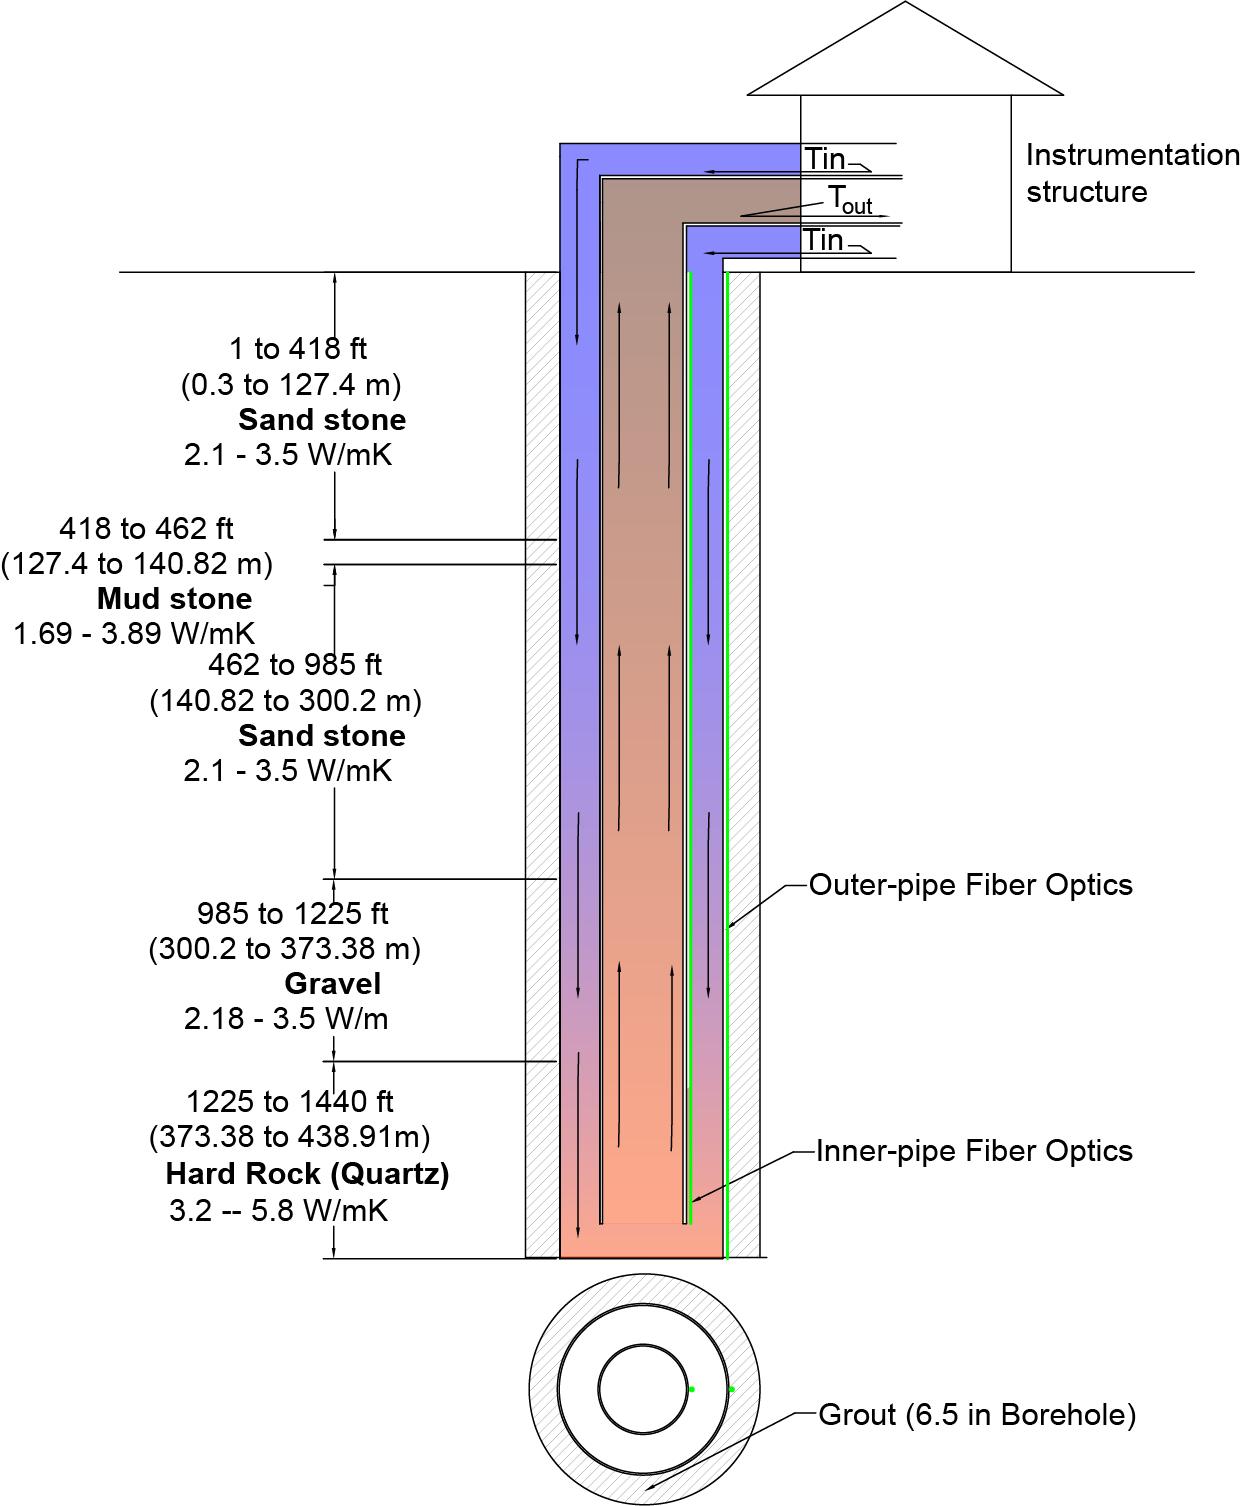
\includegraphics[height=0.5\textwidth]{data/geology_cbhe.png}
	\caption{Hydro-geological condition estimated through USGS survey immediately taken after the drilling of the well estimated at 1440 ft(438.9 m).}\label{fg:hydro}
	\end{figure}

	%Thermal conductivity variations.
	As is shown in Figure~\ref{fg:hydro}, the geological conditions around the borehole varies significantly inside the BHE. This phenomenon is not very well-represented in conventional thermal response tests.

\subsubsection{Experimental Setup}
	To characterise the thermal potentials of boreholes, thermal response tests (TRTs) are often used when estimating the borehole resistances. Following the ASHARE guidelines, the inlet and outlet temperature at the borehole are recorded. The thermal conductivity of the borehole is the mean rate of temperature change over the natural logarithmic time of either the inlet or outlet temperature beyond the initial period of heat injection. The thermal conductivities are further used to estimate the borehole resistance and other parameters to evaluate potential borehole field designs. This method clearly does not provide enough information regarding the temperature evolution along the depth of borehole, i.e. the geothermal gradient situation of individual boreholes. Recent research have pointed out possibilities to use distributed TRTs that utilise fibre optic sensors that produces depth-specific temperature measurement along the borehole.

	\begin{figure}[h!]
	\centering
	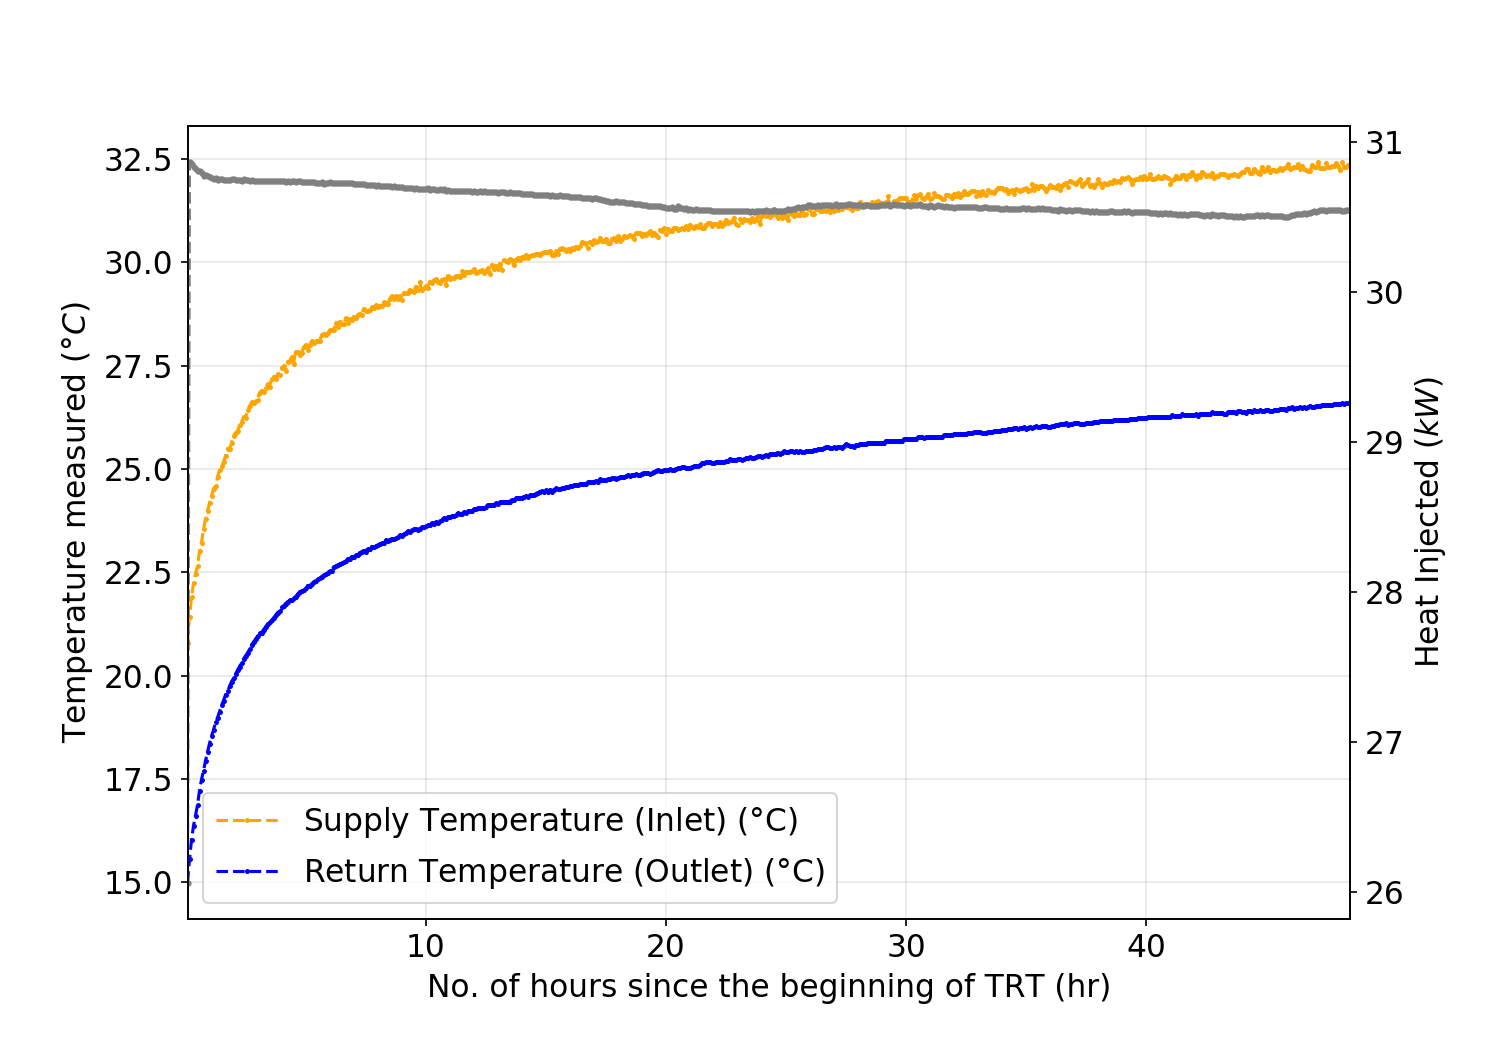
\includegraphics[width=0.65\textwidth]{data/TRT_SI}
	\caption{Temperature measured at the inlet and outlet of the well site during the thermal response test.}\label{fg:raw}
	\end{figure}

	%CBHE, Rygan, its dimensions,
	As we have previously suggested in the introduction, we are particularly interested in the effect of geothermal gradient in this study, for which we would be more interested in using coaxial borehole heat exchangers over conventional U-tube borehole heat exchangers. The CBHE option the test well project was able to procure is a Rygan borehole heat exchanger. Upon finishing the drilling and USGS geological survey, the outer pipe of the CBHE is first inserted into the test bore before it was grouted. The grout was left to set for over 24 hours until the next step of heat exchanger installation.
	A Rygan concentric heat exchanger was then installed into the drilled test bore, and grouted with a GeoPro TG select/PowerTEC 1.6, whose target thermal conductivity was 0.78W/m-K at a density of 1.2kg/L. The borehole heat exchanger has a diameter of 6.5 inch (16.5 cm) from 380 to 1340 feet. The inner diameter of the CBHE, or the OD (outer diameter) of the Rygan tube was a 2.66 inch (6.76 cm? ) and corrugated. Although this will obviously change the fluid dynamics of the flow in the annulus, we will assume the outer surface of the Rygan heat exchanger (inner tube of CBHE, not to be confused with CBHE outer tube) to be smooth within the scope of this research.


	To estimate the thermal conductivity of the formation, a thermal response test was performed on the drill site on September 10th, 2019. The test follows the guidelines recommended by the Americal Society of Heating, Refrigeration and Air-Conditioning Engineers (ASHRAE) in its HVAC Applications Handbook, Geothermal Energy Chapter. The borehole was uniformed grouted from the bottom to the top via premie pipe, and had a delay of more than five days between loop installation and test startup. The undisturbed formation temperature was estimated through the recorded temperature from the fiber optic cable installed along and around the borehole heat exchanger. The duration of the test was 48.5 hours, where the data (inlet, outlet temperature and heat injection rates) was collected every five minutes.  The heat injected was estimated to be 51 to 85 Btu/hr (or 15 to 25 W) per foot of the borehole, which averaged to be approximately 30.5 kW total heat input throughout the test. By taking the natural log time rate of change of the temperature of either the inlet and the outlet, and can be further expanded into the thermal diffusivity of the formation through an estimated heat capacity of the borehole. The estimated heat capacity of the bore can be estimated through the geological conditions previously confirmed through drilling (as shown in Figure~\ref{fg:hydro}.



	We positioned two fiber optics cable along the outer surface of both the inner and the outer pipe of the CBHE, i.e. the corrugated outer surface of the Rygan heat exchanger, and the CBHE outer tube. Fiber optic distributed temperature sensing has been previously used by many researchers to perform measurement on the therm-physical properties around boreholes in previous research(Fujii et al. 2009, Beier 2012, Acuna 2013). This is a technique that utilize the optic power measured through silica core in fiber optic cables, applying time-domain reflectometry principles and output temperatures at discrete locations adjacent to the fiber itself. Previous studies have shown the benefits of employing DTS in TRT testings, and even pointed to enhanced versions of TRT (known as DTRT) and were able to interpolate the DTS readings into depth-specific thermal conductivities(McDaniel). We installed a similar setup during our experiment, using two type-T (copper/constantan) thermocouple was attached to the data logger to monitor the reference temperature used to calibrate the readings coming in through the data logger. We used an Oryx interrogator (Sensornet, London, UK) to interpolate the data from the fiber optic cable. As the interrogator provided temperature resolution as fine as 0.01 C, and a spatial resolution as fine as 1m, we opted for various sample interval during the TRT test. During the first 10 hours of the test, we used 1 minute intervals, which was extended to 2 minutes for the subsequent measurements, including the decay test.


	The overall borehole resistance $R_b$ may therefore be estimated through Equation~\ref{eq:Rb}\cite{beier_situ_2012}. The ersulting temperature profile that may lead to the improvement of the temperature can therefore be

	\begin{equation}
		R_b = \frac{H}{Q}\{ T(t) - T_g -\frac{Q}{4\pi \lambda_g H} [E_i(\frac{r_b}{4 \alpha_g t})]   \}\label{eq:Rb}
	\end{equation}

	However, there are some inherent limitations of this method. First and foremost is the homogeneity assumption of the ground. The conventional method clearly assumes the ground to be at a homogeneous temperature along the depth of the heat exchanger, where the thermal conductivity, thermal diffusivity are also constants. However, as can be observed from Figure~\ref{fg:hydro} produced from the USGS measurement, it was clearly not the case. In particular, the hard rock or quartz at the bottom of the borehole will likely lead to a much larger thermal conductivity of the borehole, allowing the working fluid to extract more heat at the same flow rate. Within the scope of this paper, we will continue to use a single thermal conductivity calculated from the thermal response test (and the time log temperature gradient thereof) at the top of the heat exchanger to continue our analysis. However, for future research, it is desirable to expand this into a more detailed DTRT study.

	%Determined resulting thermal conductivity, rest of parameters as a table. Do we also need the thermal conductivity plot? Somewhere on the drive already I think...
